\documentclass[a4paper,10pt]{article}
\usepackage[left=1in, right=1in, top=1in, bottom=1in]{geometry}
\usepackage{graphicx}
\usepackage{array}

\begin{document}

% Header with Name and Contact Information
\begin{minipage}{0.7\textwidth}
    \textbf{\LARGE RAJJKUMAR PAL} \\
    PURSURAH,HOOGHLY,WESTBENGAL,PIN CODE- 712401 \\
    Phone: 8538031328 \\
    Email: palrajkumar2002@gmail.com
\end{minipage}
\begin{minipage}{0.3\textwidth}
    \begin{flushright}
        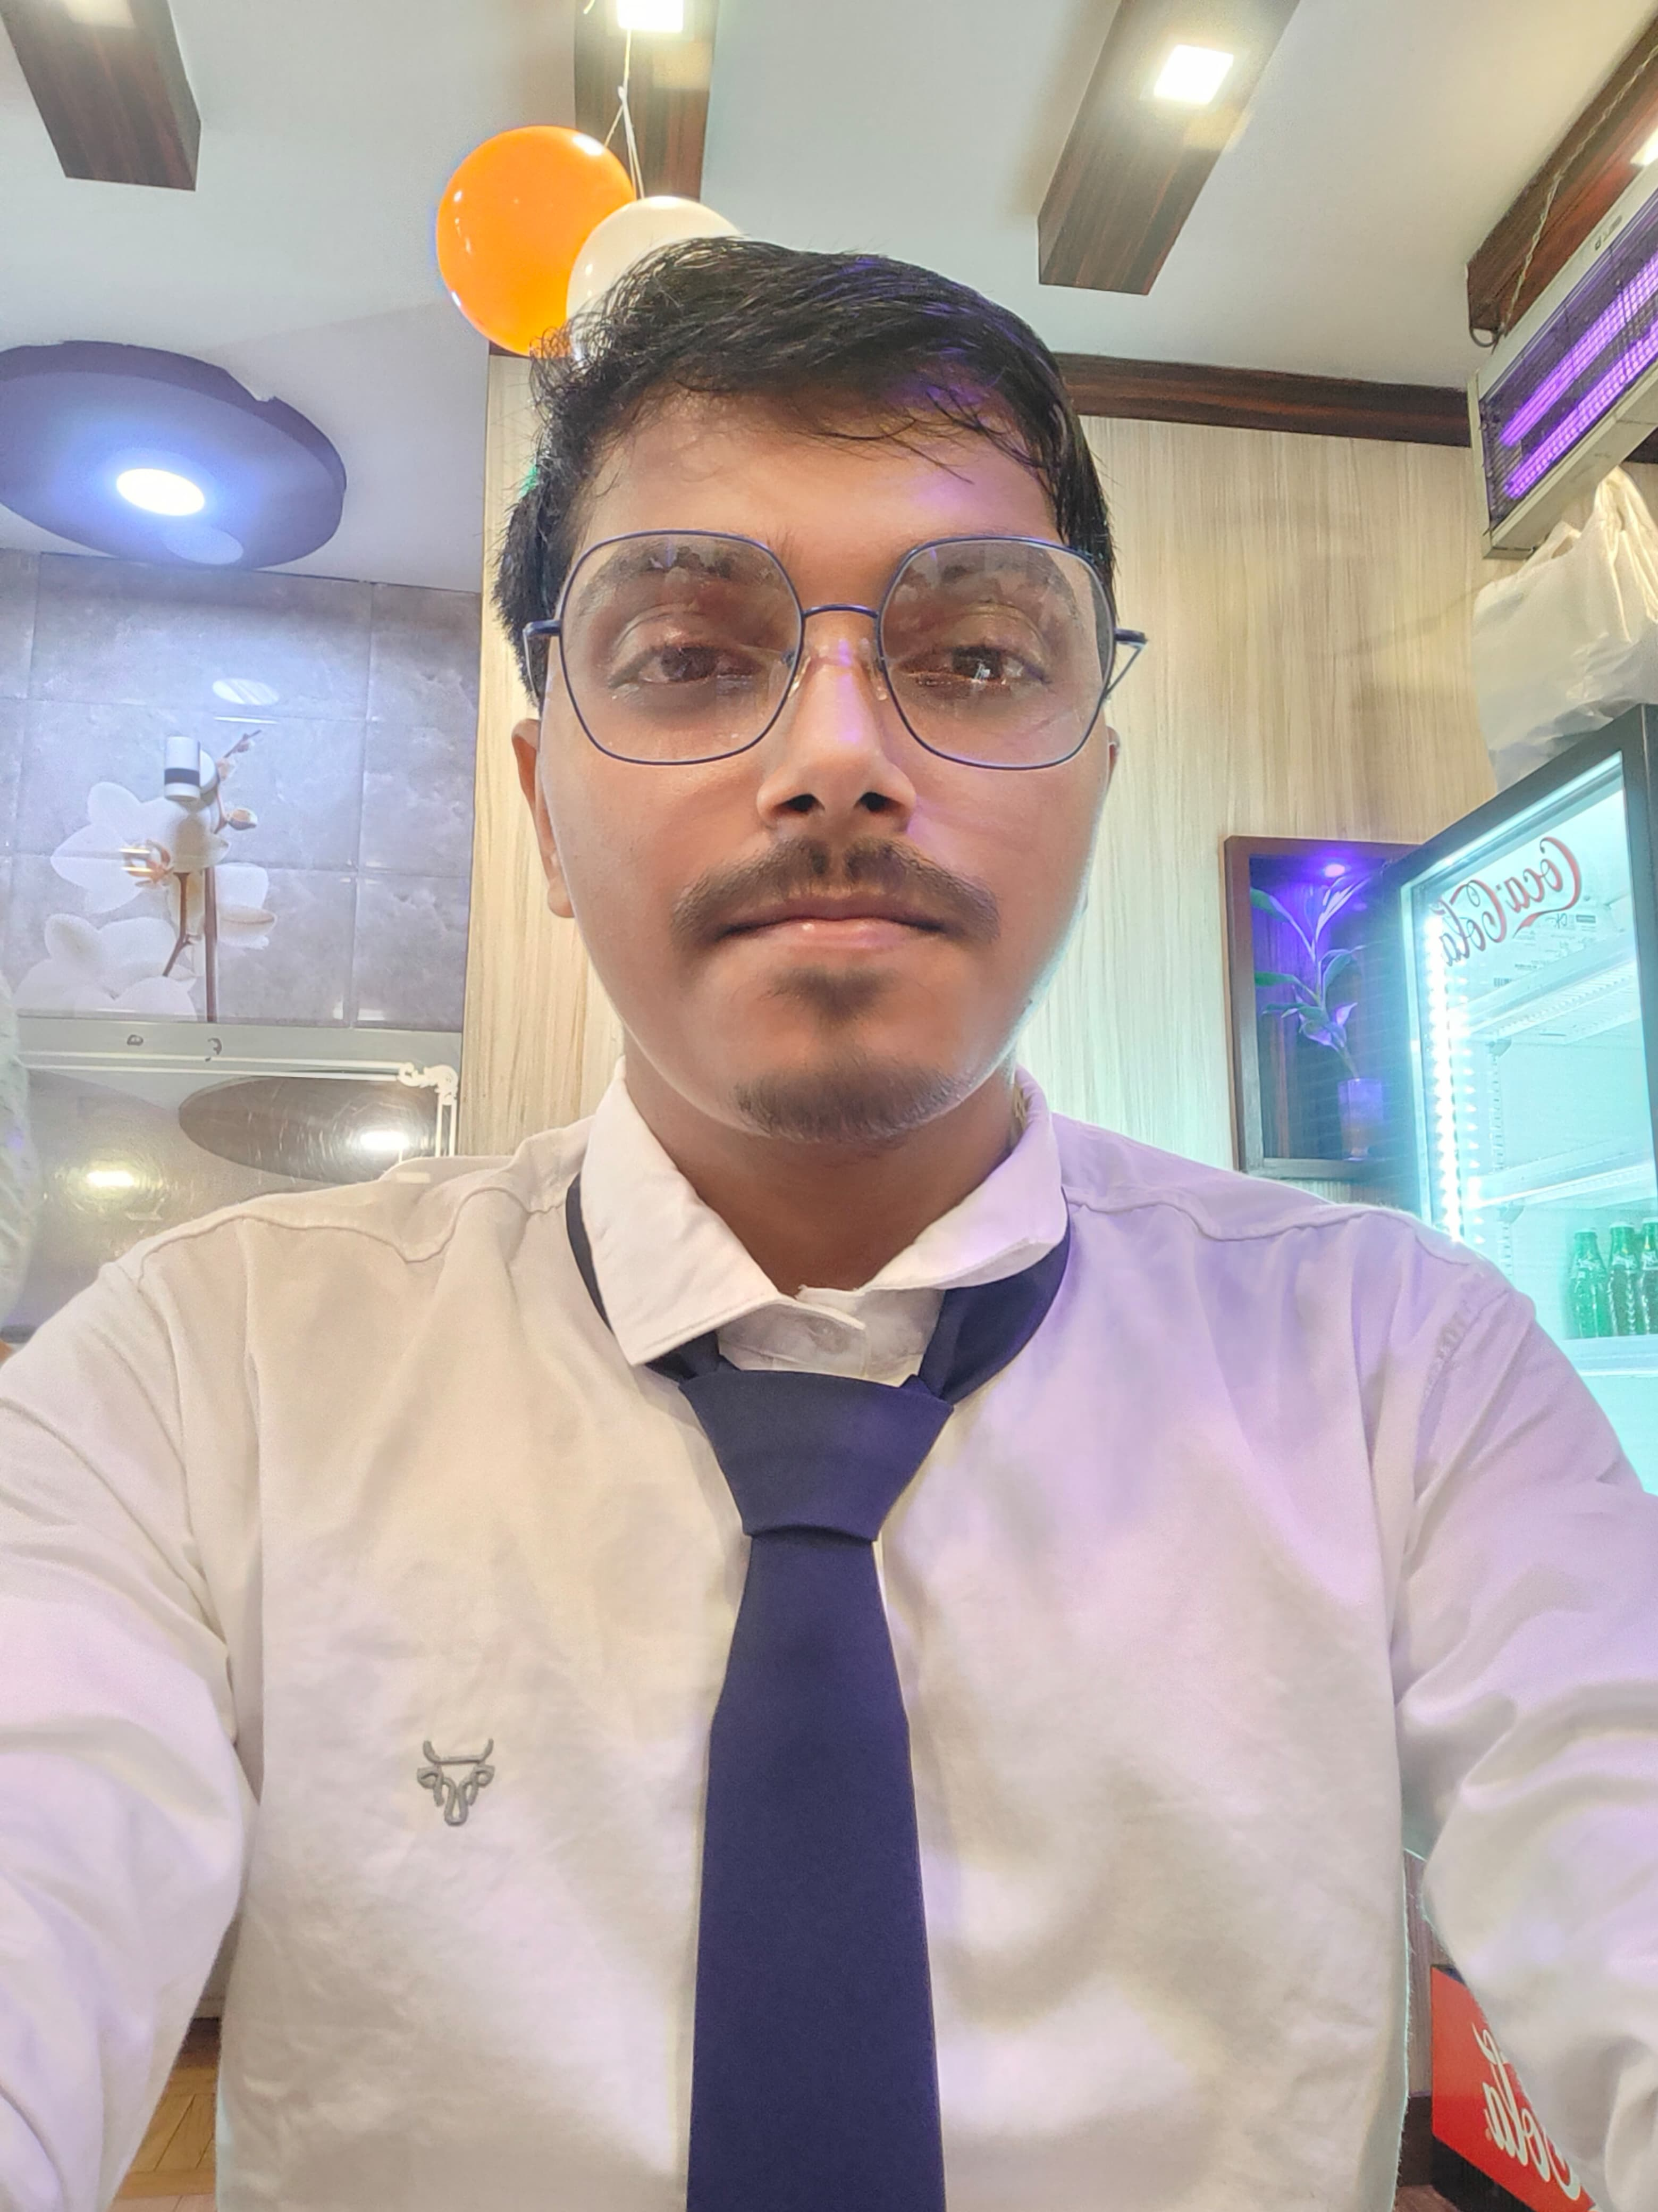
\includegraphics[width=2.5cm,height=3.5cm]{resume pic.jpg}
    \end{flushright}
\end{minipage}

\vspace{1cm}

% Education Section
\section*{Education}
\begin{tabular}{|p{5cm}|p{6cm}|p{4cm}|}
    \hline
    \textbf{Degree} & \textbf{Institution} & \textbf{Date} \\
    \hline
    BACHALOR OF COMPUTRE APPLICATION & MAULANA ABUL KALAM AZAD UNIVERSITY OF TECHNOLOGY & SEP,2023\\
    \hline
    HIGHER SECONDARY SCHOLAR  & JANGALPARA B C K M HIGH SCHOOL & MARCH,2020 \\
    \hline
\end{tabular}

\vspace{1cm}

% Awards and Achievements Section
\section*{Awards and Achievements}
\begin{itemize}
    \item SCHOLAR IN CLASS 8, JANGALPARA BCKM HIGH SCHOOL(2016) 
    \item SECONDARY SCHOLAR, JANGALPARA BCKM HIGH SCHOOL (2018)
    \item WINNER OF EXTEMPORE AT SUB-DIVISIONAL LEVEL(2028)
    \item GOT FIRST POSITION IN SINGING COMPETEION(2028)
    \item GOT SELECTED AS A JUNIOR RESEACHER IN A SPACE RESEARCH ORGANIZATION(2024)
\end{itemize}

\vspace{1cm}

% Skills Section
\section*{Skills}
\begin{itemize}
    \item \textbf{Languages:} English (Fluent), HINDI (Conversational),BENGALI(FLUENT)
    \item \textbf{Programming:} C,PYTHON
    \item \textbf{Software:} VLAB,GitHub,LaTeX,ChatGPT,MS WORD,EXCEL
    \item \textbf{EXTRA REGION OF KNOWLEDGE:} ROBOTICS AND ELECTRONICS(NEP)
     \item \textbf{INTEREST:} SINGING,DRAWING,PLAYING CHE
\end{itemize}

\end{document}
